% !TeX encoding = UTF-8

%% ------------------------------------------------------------------------
%% Copyright (C) 2021-2023 SJTUG
%% 
%% SJTUBeamer Example Document by SJTUG
%% 
%% SJTUBeamer Example Document is licensed under a
%% Creative Commons Attribution-NonCommercial-ShareAlike 4.0 International License.
%% 
%% You should have received a copy of the license along with this
%% work. If not, see <http://creativecommons.org/licenses/by-nc-sa/4.0/>.
%%
%% For a quick start, check out src/doc/sjtubeamerquickstart.tex
%% Join discussions: https://github.com/sjtug/SJTUBeamer/discussions
%% -----------------------------------------------------------------------

\documentclass[xcolor=table,dvipsnames,svgnames,aspectratio=169]{ctexbeamer}
% 可以通过 fontset=macnew / fontset=ubuntu / fontset=windows 选项切换字体集;
% 如遇无法显示的数学符号,尝试对 ctexbeamer 文档类添加 no-math 选项;
% 写纯英文幻灯片可以改用 beamer 文档类。

\usepackage{tikz}
\usepackage[normalem]{ulem}
\usetikzlibrary{arrows}
\usepackage{amsmath}
\usepackage{graphicx}
\usepackage{hologo}
\usepackage{colortbl}
\usepackage{shapepar}
\usepackage{hyperxmp}
\usepackage{booktabs}
\usepackage{listings}
\usepackage{tipa}
\usepackage{multicol}
\usepackage{datetime2}
\usepackage{fontawesome5}
\usepackage{hyperref}

% 参考文献设置,使用 style=gb7714-2015 样式为标准顺序编码制,
% 使用 style=gb7714-2015ay 样式可以改为著者-出版年制。
% \usepackage[backend=biber,style=gb7714-2015]{biblatex}
% \addbibresource{ref.bib}

% 该行指定了图像的额外搜索路径
\graphicspath{{figures/}}

\hypersetup{
  pdfcopyright       = {Licensed under CC-BY-SA 4.0. Some rights reserved.},
  pdflicenseurl      = {http://creativecommons.org/licenses/by-sa/4.0/},
  unicode            = true,
  psdextra           = true,
  pdfdisplaydoctitle = true
}

\pdfstringdefDisableCommands{
  \let\\\relax
  \let\quad\relax
  \let\hspace\@gobble
}

% \renewcommand{\TeX}{\hologo{TeX}}
% \renewcommand{\LaTeX}{\hologo{LaTeX}}
% \newcommand{\BibTeX}{\hologo{BibTeX}}
% \newcommand{\XeTeX}{\hologo{XeTeX}}
% \newcommand{\pdfTeX}{\hologo{pdfTeX}}
% \newcommand{\LuaTeX}{\hologo{LuaTeX}}
% \newcommand{\MiKTeX}{\hologo{MiKTeX}}
% \newcommand{\MacTeX}{Mac\hologo{TeX}}
% \newcommand{\beamer}{\textsc{beamer}}
% \newcommand{\XeLaTeX}{\hologo{Xe}\kern-.13em\LaTeX{}}
% \newcommand{\pdfLaTeX}{pdf\LaTeX{}}
% \newcommand{\LuaLaTeX}{Lua\LaTeX{}}
% \def\TeXLive{\TeX{} Live}
% \let\TL=\TeXLive

% \newcommand{\SJTUThesis}{\textsc{SJTUThesis}}
% \newcommand{\SJTUThesisVersion}{2.0.3}
% \newcommand{\SJTUThesisDate}{2023/9/25}
% \newcommand{\SJTUBeamer}{\textsc{SJTUBeamer}}
% \newcommand{\SJTUBeamerVersion}{3.0.0}
% \newcommand{\SJTUBeamerDate}{2022/11/22}

% \newcommand\link[1]{\href{#1}{\faLink}}
% \newcommand\pkg[1]{\texttt{#1}}

% \def\cmd#1{\texttt{\color{structure}\footnotesize $\backslash$#1}}
% \def\env#1{\texttt{\color{structure}\footnotesize #1}}
% \def\cmdxmp#1#2#3{\small{\texttt{\color{structure}$\backslash$#1}\{#2\}
% \hspace{1em}\\ $\Rightarrow$\hspace{1em} {#3}\par\vskip1em}}

\usetheme[maxplus,blue,light]{sjtubeamer}
\setbeameroption{show notes on second screen=bottom}
% 使用 maxplus/max/min 切换标题页样式
% 使用 red/blue 切换主色调
% 使用 light/dark 切换亮/暗色模式
% 使用外样式关键词以获得不同的边栏样式
%   miniframes infolines  sidebar
%   default    smoothbars split	 
%   shadow     tree       smoothtree
% 使用 topright/bottomright 切换徽标位置
% 使用逗号分隔列表以同时使用多种选项

% \setbeamertemplate{background}{}
% 对于 max 主题,如果需要关闭正文背景图,请取消注释上一行。

% \tikzexternalize[prefix=build/]
% 如果您需要缓存 tikz 图像,请取消注释上一行,并在编译选项中添加 -shell-escape。

\lstset{
  language=[LaTeX]TeX,           % 更改高亮语言
  texcsstyle=*\color{cprimary},  % 只在高亮 LaTeX 语言时必须
  tabsize=2,
  basicstyle=\ttfamily\scriptsize,%
  keywordstyle=\color{cprimary},%
  stringstyle=\color{csecondary},%
  commentstyle=\color{ctertiary!50!gray},%
  breaklines,%
}
\logo{}
\author{熊家辉}
\institute[萨塞克斯人工智能学院]{浙江工商大学}
% \date{\the\year 年 \the\month 月}
\date{2024 年 4 月 17 日}
% \date{\today}
\subject{RISCOF 初步}
\keywords{RISC-V, Architecture, Test}

\title[RISCOF 初步] % 页脚显示标题
{\textbf{RISC-V 架构测试初步}} % 首页标题

\subtitle{PLCT Lab 每周技术分享}

\begin{document}

% 使用节目录
\AtBeginSection[]{
  \begin{frame}
    %% 使用传统节目录,也可以将 subsectionstyle=... 换成 hideallsubsections 以隐藏所有小节信息
    % \tableofcontents[currentsection,subsectionstyle=show/show/hide]
    %% 或者使用节页
    \sectionpage
  \end{frame}
}

% 使用小节目录
\AtBeginSubsection[]{		       % 在每小节开始
  \begin{frame}
    %% 使用传统小节目录
    % \tableofcontents[currentsection,subsectionstyle=show/shaded/hide]
    %% 或者使用小节页
    \subsectionpage
  \end{frame}
}

\maketitle

% \begin{frame}
%   \frametitle{来源}
%   \begin{thebibliography}{00}
%     \setbeamertemplate{bibliography item}[online]
%     \bibitem{} Alexara Wu.
%     \newblock 如何使用 \LaTeX{} 排版论文[EB/OL].
%     \newblock 2021.
%     \url{https://github.com/sjtug/sjtulib-latex-talk/tree/alexara-2021}
%   \end{thebibliography}

%   \vspace*{2ex}

%   \begin{itemize}
%     \item 本示例文档的源码结构适用于简短的单次报告,仅展示 \beamer{} 文档类的通
%           用功能,更多地在使用 \SJTUBeamer{} 的样式信息。
%     \item 为发挥 \SJTUBeamer{} 的全部功能,参见发布区
%           \link{https://github.com/sjtug/SJTUBeamer/releases} 的快速入门、用户手
%           册与开发文档。
%     \item 就制作一组讲座而言,相关源码结构可以参考新讲座
%           \link{https://github.com/sjtug/sjtulib-latex-talk/tree/logcreative-2022}。
%           新讲座使用了社区版主题的同时也展示了 \SJTUBeamer{} 的特殊用法。
%   \end{itemize}

% \end{frame}

% \begin{frame}{目录}
%   \tableofcontents[hideallsubsections]	% 隐藏所有小节信息
% \end{frame}

\section{简介}

\subsection{riscv-arch-test 简介}

\begin{frame}
  \frametitle{项目链接}

  \href{https://github.com/riscv-non-isa/riscv-arch-test}{riscv-non-isa/riscv-arch-test} 是 RISC-V 基础架构测试 SIG 工作的存储库。

  希望自我证明其实现与 RISC-V 兼容的供应商可以在此 \href{https://github.com/riscv-non-isa/riscv-arch-test-reports}{riscv-non-isa/riscv-arch-test-reports} 存储库中存档其测试结果。
\end{frame}

\begin{frame}%[fragile]
  \frametitle{项目目的}
  RISC-V 架构测试是一组不断发展的测试,旨在帮助确保为给定 RISC-V 配置文件/规范编写的软件能够在符合该配置文件的所有实现上运行。

  这些测试还有助于确保实施者正确理解并实施了规范。通过 RISC-V 架构测试并不意味着设计符合 RISC-V 架构。 这些只是一组基本的测试,检查规范的重要方面,而不关注细节。

  RISC-V 架构测试不能替代严格的设计验证。架构测试向用户提供的结果可以保证规范已被正确解释,并且被测实现 (DUT) 可以被声明为符合 RISC-V 架构测试。
\end{frame}

\begin{frame}
  \frametitle{项目内容}
  \begin{itemize}
    \item doc: 项目的所有文档,使用AsciiDoc编写。
    \item coverage: 该目录包含多个覆盖点 YAML,它们捕获 riscv-test-suite 目录中的所有测试覆盖的所有感兴趣的覆盖点。
    \item riscv-test-suite: 其中包括在套件中的测试中使用的通用汇编宏和例程。 还有更多目录包含实际的架构测试。
  \end{itemize}

  \note{coverage 文件夹里面包含了很多cgf文件。该文件描述了对于某一个指定的扩展,需要覆盖到的寄存器、指令}
\end{frame}

\subsection{RISCOF 简介}

\begin{frame}
  \frametitle{RISCOF 简介}
  RISCOF:RISC-V 兼容性框架是一个基于 Python 的框架,可使用一套 RISC-V 架构组装测试针对标准 RISC-V 黄金参考模型测试 RISC-V 目标(硬或软实现)。
\end{frame}

\begin{frame}<1-2>
  \frametitle{RISCOF 简介}
  \begin{figure}
    \centering
    \begin{stampbox}
      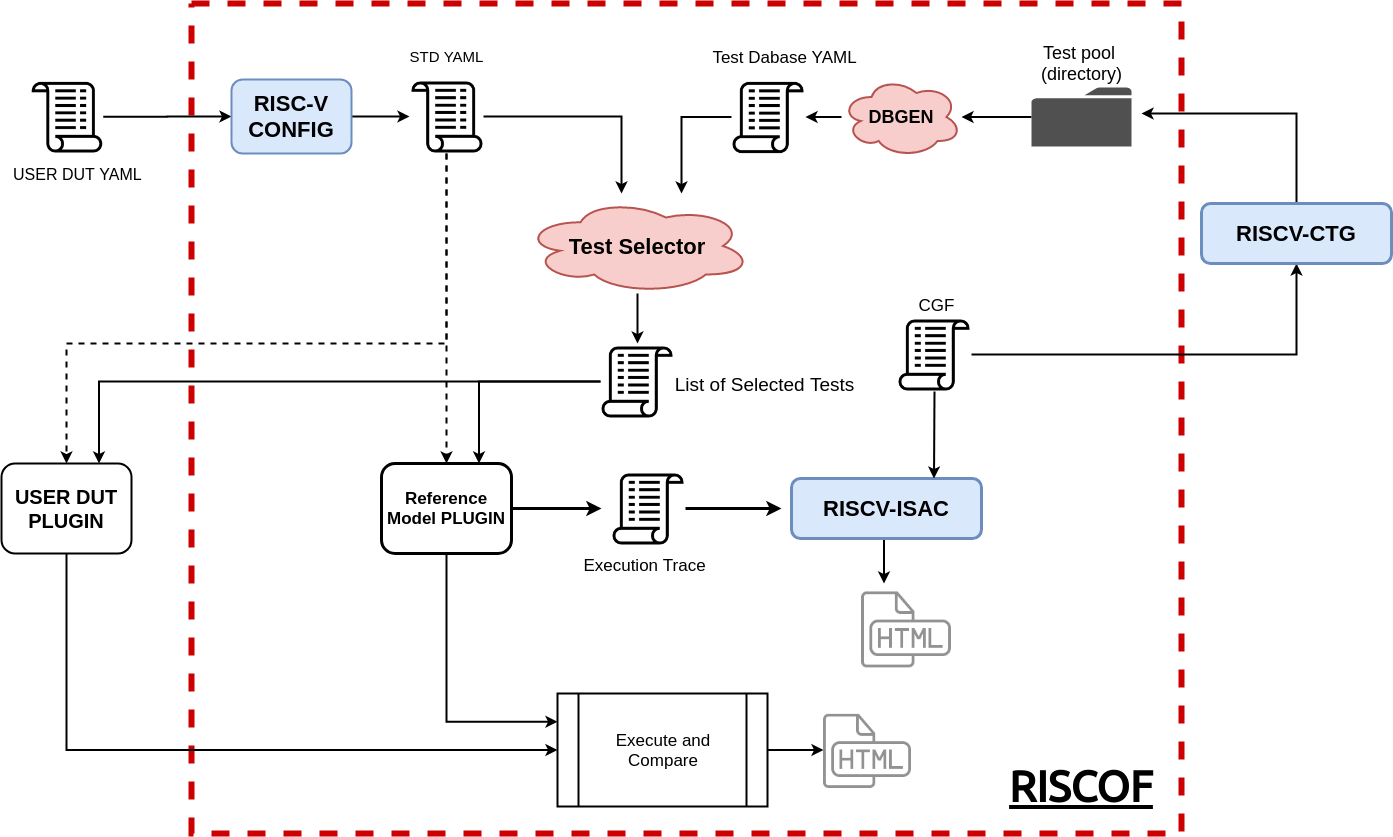
\includegraphics
      [height=.5\textheight]
      {figures/riscof.png}
    \end{stampbox}
    \caption{RISCOF 组件}
  \end{figure}
  \note<1>[item]{用户做出的 ISA 选择的基于 RISCV-CONFIG 的 YAML 规范。
    \item 一个 Python 插件,框架可以使用它来编译测试、模拟测试并提取每个测试的签名。构建模型插件部分提供了定义 python 插件的步骤。
    \item RISCV-CONFIG:需要该工具来验证用户提供的输入ISA YAML的合法性。
    \item RISCV-ISAC:该工具用于提供覆盖率分析以及对当今 RISCOF 中可用架构套件的质量评估。
    \item RISCV-CTG:RISCV-CTG 是基于 RISC-V 的兼容性测试生成器。
  }
  \note<2>[item]{DBGEN:RISCOF 在内部维护架构测试套件中所有可用组装测试的数据库。 该数据库以 YAML 文件形式维护,用于为给定 DUT 模型选择相关测试。 DBGEN 根据 RISCOF 中可用的测试自动生成此 YAML 文件。该实用程序的目标是供测试贡献者使用其新测试更新数据库。 有关其功能和用法的更多信息,请参阅数据库生成器
    \item 测试选择器:随着 RISCOF 的发展,RISCOF 将包含大量的架构测试。 然而,并非所有测试都适用于 RISC-V 目标的给定配置。 因此,测试选择器实用程序使用来自用户的标准化 RISCV-CONFIG 规范和测试数据库来过滤和仅选择那些适用于所考虑的 RISC-V 目标的测试。 此列表以 YAML 文件形式呈现,有关此格式的更多信息可在测试列表格式中找到。   该实用程序目前是 RISCOF 内部的,不能作为单独的 cli(命令行界面)使用。 用户或贡献者都不需要将此实用程序作为单独的模块来处理。
  }
\end{frame}

\section{RISCOF 运行}

\subsection{依赖准备}

\begin{frame}
  \frametitle{依赖安装}
  \begin{itemize}
    \item Python
    \item RISCV-GNU Toolchain:一个工具链。
    \item 两个插件
  \end{itemize}
\end{frame}

\begin{frame}[fragile]
  \frametitle{构造工具链}

  编译工具链的详细过程请参阅 \href{https://github.com/ArielHeleneto/Work-PLCT/blob/master/help/build-riscv-toolchain.md}{在国内网络环境下编译 riscv-gnu-toolchain}。选用镜像也不错。

  \begin{codeblock}[language=bash]{工具链编译}
git clone --recursive https://github.com/riscv/riscv-gnu-toolchain
git clone --recursive https://github.com/riscv/riscv-opcodes.git
cd riscv-gnu-toolchain
./configure --prefix=/path/to/install --with-arch=rv32gc --with-abi=ilp32d
make
  \end{codeblock}

  确认当前 PATH 内包含 \lstinline|riscv32-unknown-elf-\*|。
\end{frame}

\begin{frame}
  \frametitle{插件简介}

  在当前情况下,Spike 将充当待测部件,Sail 将充当参考部件。

  \begin{columns}[T]
    \begin{column}{.5\textwidth}
      \alert{\textbf{Sail C 模拟器}}
      \stamphrule
      一个用 Sail 写的模拟器,参见 \href{https://github.com/riscv/sail-riscv.git}{sail-riscv}。
      该模拟器包含用 Sail 编写的 RISC-V 架构的正式规范。它已被 RISC-V 基金会采用。该模型规定了指令的汇编语言格式、相应的编码器和解码器以及指令语义。
    \end{column}
    \textcolor{cprimary}{\vrule}\hfill
    \begin{column}{.5\textwidth}
      \alert{\textbf{Spike}}
      \stamphrule
      Spike, 参见 \href{https://github.com/riscv-software-src/riscv-isa-sim.git}{riscv-isa-sim}。Spike 是没有头图 RISC-V ISA 模拟器,可实现一个或多个 RISC-V hart 的功能模型。
    \end{column}
  \end{columns}

\end{frame}

\begin{frame}[fragile]
  \frametitle{构造工具链}

  编译工具链的详细过程请参阅 \href{https://github.com/ArielHeleneto/Work-PLCT/blob/master/help/build-riscv-toolchain.md}{在国内网络环境下编译 riscv-gnu-toolchain}。选用镜像也不错。

  \begin{codeblock}[language=bash]{工具链编译}
git clone --recursive https://github.com/riscv/riscv-gnu-toolchain
git clone --recursive https://github.com/riscv/riscv-opcodes.git
cd riscv-gnu-toolchain
./configure --prefix=/path/to/install --with-arch=rv32gc --with-abi=ilp32d
make
  \end{codeblock}

  确认当前 PATH 内包含 \lstinline|riscv32-unknown-elf-\*|。
\end{frame}

\begin{frame}[fragile,allowframebreaks]
  \frametitle{构造 Sail}

  \begin{codeblock}[language=bash]{Sail 依赖}
sudo apt-get install opam  build-essential libgmp-dev z3 pkg-config zlib1g-dev
opam init -y --disable-sandboxing
opam switch create ocaml-base-compiler.4.06.1
opam install sail -y
eval \$(opam config env)

  \end{codeblock}
  \begin{codeblock}[language=bash]{构建 Sail}
git clone https://github.com/riscv/sail-riscv.git
cd sail-riscv
make
ARCH=RV32 make
ARCH=RV64 make
ln -s sail-riscv/c_emulator/riscv_sim_RV64 /usr/bin/riscv_sim_RV64
ln -s sail-riscv/c_emulator/riscv_sim_RV32 /usr/bin/riscv_sim_RV32
  \end{codeblock}
\end{frame}

\begin{frame}[fragile]
  \frametitle{使用 Docker Sail}

  \begin{codeblock}[language=bash]{Docker Sail}
docker pull registry.gitlab.com/incoresemi/docker-images/compliance
  \end{codeblock}

\end{frame}

\subsection{准备配置}

\begin{frame}
  \frametitle{插件介绍}

  RISCOF 提供了多个模板用作基础配置文件。

  \begin{itemize}
    \item \href{https://gitlab.com/incoresemi/riscof-plugins/-/tree/master/spike_parallel}{Spike}
    \item \href{https://gitlab.com/incoresemi/riscof-plugins/-/blob/master/sail_cSim/}{SAIL\_cSim}
    \item \href{https://gitlab.com/incoresemi/riscof-plugins}{InCore Plugins}:这是一组插件。
    \item \href{https://github.com/stnolting/neorv32-riscof}{neorv32 Plugins}:第三方插件,供 neorv32 使用。
  \end{itemize}

  \note{neorv32 是个微型、可定制和可扩展的 MCU 级 32 位 RISC-V 软核 CPU 和用独立于平台的 VHDL 编写的类似微控制器的 SoC。RV32 [I/E] [M] [A] [C] [B] [U] [X] [Zicsr] [Zicntr] [Zicond] [Zihpm] [Zifencei] [Zfinx] [Zmmul] [Zxcfu] [Smpmp] [Sdext] [Sdtrig]}

\end{frame}

\begin{frame}[fragile,allowframebreaks]
  \frametitle{生成配置文件}

  \begin{codeblock}[language=bash]{生成配置文件}
riscof setup --dutname=spike
  \end{codeblock}

  该命令产生一组配置文件用于控制架构测试。

  \begin{codeblock}[language=bash]{成功生成配置文件}
INFO | ****** RISCOF: RISC-V Architectural Test Framework 1.25.3 *******
INFO | using riscv_isac version : 0.18.0
INFO | using riscv_config version : 3.18.1
INFO | Setting up sample plugin requirements [Old files will be overwritten]
INFO | Creating sample Plugin directory for [DUT]: spike
INFO | Creating sample Plugin directory for [REF]: sail_cSim
INFO | Creating Sample Config File
INFO | **NOTE**: Please update the paths of the reference and plugins in the config.ini file
  \end{codeblock}

  \newpage

  配置文件为 \lstinline|config.ini|。

  \begin{codeblock}{Spike 插件清单}
spike/ # 待测元件
  env
    link.ld # 待测元件描述文件
    model_test.h # 待测元件头文件
  riscof_spike.py # 插件
  spike_isa.yaml # 待测元件 ISA 描述
  spike_platform.yaml # 待测元件平台描述
  \end{codeblock}
  \begin{codeblock}{Sail 插件清单}
sail_cSim/ # 参考模型
  env
    link.ld # 参考元件描述文件
    model_test.h # 待测元件头文件
  __init__.py
  riscof_sail_cSim.py # 插件
      \end{codeblock}
\end{frame}

\begin{frame}[fragile,allowframebreaks]
  \frametitle{设置配置文件}
  \begin{codeblock}{配置文件正文}
[RISCOF]
ReferencePlugin=sail_cSim
ReferencePluginPath=/home/ariel/riscof/sail_cSim
DUTPlugin=spike
DUTPluginPath=/home/ariel/riscof/spike
  \end{codeblock}
  \newpage
  \begin{codeblock}{spike配置}
[spike]
pluginpath=/home/ariel/riscof/spike
ispec=/home/ariel/riscof/spike/spike_isa.yaml
pspec=/home/ariel/riscof/spike/spike_platform.yaml
target_run=1
  \end{codeblock}
  \newpage
\begin{codeblock}{编译的 Sail 配置}
[sail_cSim]
pluginpath=/home/ariel/riscof/sail_cSim
PATH=/path/to/install/riscv_sim_RV64
  \end{codeblock}
  \begin{codeblock}{Docker Sail 配置}
[sail_cSim]
pluginpath=/path/to/riscof/sail_cSim
docker=True
image=registry.gitlab.com/incoresemi/docker-images/compliance
  \end{codeblock}
  
\end{frame}

\begin{frame}[fragile]
  \frametitle{展开架构测试}

  \begin{codeblock}[language=bash]{riscv-arch-test}
riscof --verbose info arch-tests --clone
  \end{codeblock}

\end{frame}

\subsection{运行}

% \begin{frame}[fragile]
%   \frametitle{检查配置文件}

%   第一步是检查输入的 yaml 文件是否配置正确。

%   \begin{codeblock}[language=bash]{工具链编译}
% riscof validateyaml --config=config.ini
%   \end{codeblock}

% \end{frame}

\begin{frame}[fragile,allowframebreaks]
  \frametitle{运行架构测试}

  第一步是检查输入的 yaml 文件是否配置正确。

  \begin{codeblock}[language=bash]{检查输入}
riscof validateyaml --config=config.ini
  \end{codeblock}
  \begin{codeblock}{YAML 文件验证}
[INFO]    : Reading configuration from: /scratch/git-repo/incoresemi/riscof/config.ini
[INFO]    : Preparing Models
[INFO]    : Input-ISA file
[INFO]    : Loading input file: /scratch/git-repo/incoresemi/riscof/spike/sample_isa.yaml
[INFO]    : Load Schema /home/neel/.pyenv/versions/3.7.0/envs/venv/lib/python3.7/site-packages/riscv_config/schemas/schema_isa.yaml
[INFO]    : Initiating Validation
  \end{codeblock}
  % [INFO]    : No Syntax errors in Input ISA Yaml. :)
% [INFO]    : Dumping out Normalized Checked YAML: /scratch/git-repo/incoresemi/riscof/riscof_work/sample_isa_checked.yaml
% [INFO]    : Input-Platform file
% [INFO]    : Loading input file: /scratch/git-repo/incoresemi/riscof/spike/sample_platform.yaml
% [INFO]    : Load Schema /home/neel/.pyenv/versions/3.7.0/envs/venv/lib/python3.7/site-packages/riscv_config/schemas/schema_platform.yaml
% [INFO]    : Initiating Validation
% [INFO]    : No Syntax errors in Input Platform Yaml. :)
% [INFO]    : Dumping out Normalized Checked YAML: /scratch/git-repo/incoresemi/riscof/riscof_work/sample_platform_checked.yaml
\end{frame}

\begin{frame}[fragile,allowframebreaks]
  \frametitle{选中测试}

  第二步是生成测试用例表。

  \begin{codeblock}[language=bash]{生成测试用例表}
riscof testlist --config=config.ini --suite=riscv-arch-test/riscv-test-suite/ --env=riscv-arch-test/riscv-test-suite/env
  \end{codeblock}
  \begin{codeblock}[language=bash]{选中用例}
[INFO]    : Selecting Tests.
  \end{codeblock}

  选中的测试会列在 \lstinline|riscof_work/test_list.yaml|。

  \begin{codeblock}{用例表样式}
suite/rv32i_m/C/C-ADD.S:
  work_dir: /scratch/git-repo/incoresemi/riscof/riscof_work/rv32i_m/C/C-ADD.S
  macros: [TEST_CASE_1=True, XLEN=32]
  isa: RV32IC
  test_path: /home/neel/.pyenv/versions/3.7.0/envs/venv/lib/python3.7/site-packages/riscof/suite/rv32i_m/C/C-ADD.S
  \end{codeblock}

\end{frame}

\begin{frame}[fragile,allowframebreaks]
  \frametitle{运行测试}

  第三步是运行测试。

  \begin{codeblock}[language=bash]{工具链编译}
riscof run --config=config.ini --suite=riscv-arch-test/riscv-test-suite/ --env=riscv-arch-test/riscv-test-suite/env
  \end{codeblock}
  \begin{codeblock}[language=bash]{工具链编译}
[INFO]    : Initiating signature checking.
[INFO]    : Following 55 tests have been run :
[INFO]    : TEST NAME                                          : COMMIT ID                                : STATUS
[INFO]    : suite/rv32i_m/I/I-ADD-01.S                         : d50921ef64708678832770fd842355aa2b0684af : Passed
[INFO]    : suite/rv32i_m/I/I-ADDI-01.S                        : d50921ef64708678832770fd842355aa2b0684af : Passed
  \end{codeblock}

  输出到 \lstinline|riscof_work/report.html|。
\end{frame}

\begin{frame}[fragile,allowframebreaks]
  \frametitle{覆盖率检查}

  这是可选步骤。该步骤生成了覆盖率报告。

  \begin{codeblock}[language=bash]{生成覆盖率报告}
riscof --verbose debug coverage --suite /path/to/suite --env /path/to/suite
  \end{codeblock}
  % INFO | [--root--]: Reading configuration from: /home/neel/temp/config.ini
% INFO | [--root--]: Preparing Models
% INFO | [--riscv_config.checker--]: Input-ISA file
% INFO | [--riscv_config.checker--]: Loading input file: /home/neel/temp/riscof-plugins/spike/spike_isa.yaml
% INFO | [--riscv_config.checker--]: Load Schema /home/neel/.pyenv/versions/3.7.0/envs/venv/lib/python3.7/site-packages/riscv_config/schemas/schema_isa.yaml
% INFO | [--riscv_config.checker--]: Processing Hart: hart0
% INFO | [--riscv_config.checker--]: Initiating Validation
% INFO | [--riscv_config.checker--]: No errors for Hart: 0 :)
% INFO | [--riscv_config.checker--]: Initiating post processing and reset value checks.
% INFO | [--riscv_config.checker--]: Dumping out Normalized Checked YAML: /home/neel/temp/riscof_work/spike_isa_checked.yaml
% INFO | [--riscv_config.checker--]: Input-Platform file
% INFO | [--riscv_config.checker--]: Loading input file: /home/neel/temp/riscof-plugins/spike/spike_platform.yaml
% INFO | [--riscv_config.checker--]: Load Schema /home/neel/.pyenv/versions/3.7.0/envs/venv/lib/python3.7/site-packages/riscv_config/schemas/schema_platform.yaml
% INFO | [--riscv_config.checker--]: Initiating Validation
% INFO | [--riscv_config.checker--]: No Syntax errors in Input Platform Yaml. :)
% INFO | [--riscv_config.checker--]: Dumping out Normalized Checked YAML: /home/neel/temp/riscof_work/spike_platform_checked.yaml
% INFO | [--root--]: Will collect Coverage using RISCV-ISAC
% INFO | [--root--]: CGF file being used : /scratch/git-repo/incoresemi/riscof/riscof/suite/compliance.cgf
% INFO | [--riscof.framework.test--]: Selecting Tests.
% INFO | [--riscof.framework.main--]: Running Tests on Reference.
% INFO | [--riscof.framework.main--]: Merging Coverage reports

%INFO | [--root--]: Openning test report in web-browser
  \begin{codeblock}[language=bash]{工具链编译}
INFO | [--root--]: Test report generated at /home/neel/temp/riscof_work/coverage.html.
  \end{codeblock}

  输出到 \lstinline|riscof_work/coverage.html|。
\end{frame}

\section{RISCV-CTG}

\subsection{RISCV-CTG 简介}

\begin{frame}
  \frametitle{项目链接}

  \href{https://github.com/riscv-software-src/riscv-ctg}{riscv-software-src/riscv-ctg} 是基于 RISC-V 的兼容性测试生成器。该工具用于生成官方 RISC-V 架构测试套件和 RISC-V 架构测试框架 RISCOF 中使用的测试。 CTG 生成的所有测试均符合官方测试格式规范。

  CTG 类似于约束测试生成器,能够生成针对特定约束集的测试。 这些约束使用覆盖组格式 (CGF) 文件提供给 CTG。 CGF 文件包含不同指令的各种覆盖点。 CTG 将每个覆盖点视为约束,并使用求解器来识别潜在的解决方案。 CTG 使用 python-constraint 包提供的约束满足问题 (CSP) 求解器。
\end{frame}

\begin{frame}%[fragile]
  \frametitle{项目目的}
  CTG 的目标用户/受众是验证和设计工程师,他们希望创建一套专注于覆盖特定极端情况的测试。 然后可以使用这些测试来展示指令本身的功能。

  请注意,CTG 的功能完全受到 CGF 中覆盖点的限制。 可以向 CTG 提供涵盖指令所有极端情况的更精细的 CGF,以便为该指令创建近似验证测试。
\end{frame}

\begin{frame}<1-3>
  \frametitle{RISCV-CTG 组件}
  \begin{figure}
    \centering
    \begin{stampbox}
      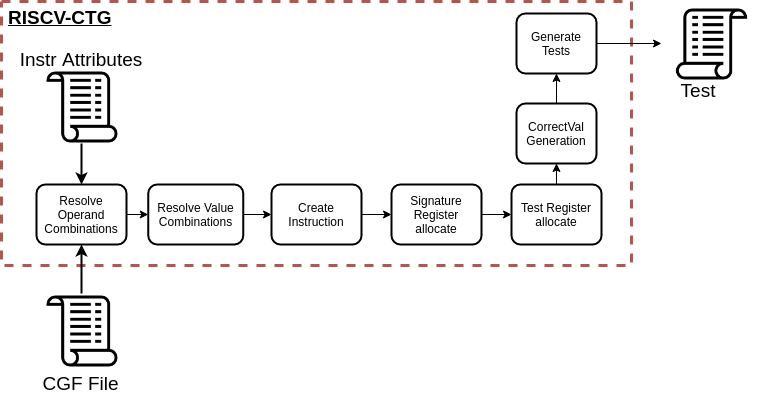
\includegraphics
      [height=.5\textheight]
      {figures/riscctg.png}
    \end{stampbox}
    \caption{RISCV-CTG 组件}
  \end{figure}

  \note[item]<1>{Instr Attributes: 为了生成给定指令的测试,需要事先知道指令的属性。 此信息以 YAML 格式存储在 CTG 中,称为属性文件。
  \item Op and Val Combinations:CTG 的前两个阶段接收输入 CGF 文件并识别操作数和值组合的解决方案。 这些解决方案是相互独立执行的。 在这些阶段中,求解器用于寻找满足相应覆盖点的解决方案。 此处还分配了立即值。如果启用随机化,则使用随机求解器。
  \item Instruction Creation:本阶段将前几个阶段导出的操作数和值组合解在本阶段相互组合,完成待测指令的所有字段。
  }
  \note<2>[item]{Signature and Test Register Allocation:还应该为指令的每个实例提供一个签名寄存器来保存操作结果,以及一个附加的测试寄存器来执行备用的特定于目标的检查或调试。寄存器以贪婪方式分配,使得最大数量的指令使用相同的签名和测试寄存器。 因此,这导致寄存器之间的指针传输最少。
  \item CorrectVal Generation:对于一些算术指令,如 add、sll、sub 等,可以轻松定义属性 YAML 中相应的操作字段来捕获这些指令的行为。 在此,CTG 阶段使用这些字段来定义这些操作的预期值/结果。 测试中的这些 Correctval 字段可用于执行结果的内联检查和调试失败。(还在开发)
  \item Generate Tests:最后,定义所有字段后,使用符合测试格式规范的特定测试模板来生成每条指令的汇编文件。
  }
  \note<3>{由于 CTG 采用 CSP 求解器,涉及大型数据集的某些约束的运行时间可能很快就会增加。 CTG 通常还用于生成跨指令的一套测试,而不是单个测试。 因此,为了减少套件生成的运行时间,CTG 在内部将 CGF 中的覆盖组分配给单个主机进程,从而并行运行。
  随机求解器对于提高速度至关重要。 由于 CGF 中定义松散的约束(例如 rs1\_val \> 0 和 rs2\_val \> 0),当数据集很大时,求解器可能会花费相当长的时间来找到所有解决方案。 另一方面,随机求解器提供第一个满足问题的解决方案,然后退出,从而节省时间。
  
  对松散定义的约束使用随机值的第二个好处是,它增加了在同一指令中覆盖多个覆盖点(稍后可能会介绍)的机会。 因此,这减少了覆盖 CGF 覆盖组中提到的所有覆盖点所需的指令数量。
  
  必须注意的是,测试的覆盖范围绝不会因为使用随机求解器而受到影响。
  
  使用随机求解器的一个明显缺点是无法再次重现相同的测试。 然而,CTG 用户的典型意图是生成满足 CGF 中定义的覆盖点的测试。 由于这是由 CTG 保证的,所以可重复性问题可以放在一边。}
\end{frame}

\begin{frame}[fragile]
  \frametitle{Instr Attributes}

  \begin{codeblock}{CTG 属性文件}
add:
  xlen: [32,64]
  isa: I
  operation: 'hex((rs1_val + rs2_val) & (2**(xlen)-1))'
  formattype: 'rformat'
  rs1_op_data: *all_regs
  rs2_op_data: *all_regs
  rd_op_data: *all_regs
  rs1_val_data: 'gen_sign_dataset(xlen) + gen_sp_dataset(xlen,True)'
  rs2_val_data: 'gen_sign_dataset(xlen) + gen_sp_dataset(xlen,True)'
  template: TEST_RR_OP(\$inst, \$rd, \$rs1, \$rs2, \$correctval, \$rs1_val, \$rs2_val, \$swreg, \$offset, \$testreg)
  \end{codeblock}
\note[item]{name:指令名称
\item xlen: 该指令适用的 XLEN 值列表
\item isa: 该指令属性所属的RISC-V ISA扩展
\item operation:一个Python计算的字符串,它定义了指令的功能
\item formattype: 指示指令格式类型的字符串
\item rs1\_op\_data: 可用作操作数 1 的合法寄存器列表
\item rs2\_op\_data: 可用作操作数 2 的合法寄存器列表
\item rd\_op\_data: 可用作目标的合法寄存器列表
\item rs1\_val\_data: 可用作操作数 1 的值的整数列表
\item rs2\_val\_data: 可用作操作数 2 的值的整数列表
\item template: 一个字符串,指示用于创建测试的汇编宏。}
\note{// opcode: \$inst ; op1:\$rs1; op2:\$rs2; dest:\$rd; op1val:\$rs1\_val;  op2val:\$rs2\_val
}
\end{frame}

\section{RISCV-Config}

\subsection{RISCV-Config 简介}

\begin{frame}
  \frametitle{项目链接}

  \href{https://github.com/riscv/riscv-config}{riscv/riscv-config} RISCV-Config 是用于生成标准化描述文件的工具。

\end{frame}

\begin{frame}%[fragile]
  \frametitle{项目目的}
  该工具用于确定唯一的描述文件,用于描述目标 ISA 和用户实现的平台特定功能。 
\end{frame}

\begin{frame}
  \frametitle{RISCV-Config 组件}
  \begin{figure}
    \centering
    \begin{stampbox}
      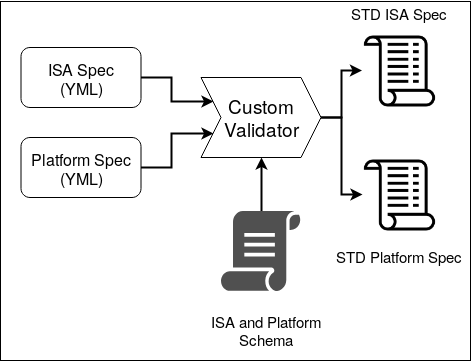
\includegraphics
      [height=.5\textheight]
      {figures/riscv_config-flow.png}
    \end{stampbox}
    \caption{RISCV-Config 组件}
  \end{figure}

  \note[item]{ISA 规范:此 YAML 文件旨在捕获用户实现的 ISA 相关功能。 该输入文件的详细信息可以在这里找到:ISA YAML Spec。
  \item 平台规范:此 YAML 文件旨在捕获用户实现的平台特定功能。 此输入文件的详细信息可以在此处找到:Platform YAML Spec。}
  \note{验证器首先检查 ISA 和平台规范是否存在不一致之处。 像“F”("F"即单精度浮点(single-precision floating-point)这样的检查是否存在“D”(双精度浮点指令(依赖于基本的单精度浮点指令子集F))是由验证者执行的。D扩展依赖F扩展。 如果为规范提供了任何非法配置,验证器将退出并显示错误。 一旦验证器检查通过,就会生成两个单独的标准 yaml 文件,每个文件对应一种输入类型。 这些标准 yaml 文件包含每个节点的所有详细字段和附加信息。 虽然用户不需要指定输入 yaml 文件中的所有字段,但验证器将为这些字段分配默认值,并为 ISA 和平台规范生成标准的详尽 yaml。}
\end{frame}

\section{RISC-V ISA Coverage}

\subsection{RISC-V ISAC 简介}

\begin{frame}
  \frametitle{项目链接}

  \href{https://github.com/riscv/riscv-isac}{riscv/riscv-isac} 用于提供覆盖率分析以及对当今 RISCOF 中可用架构套件的质量评估。

\end{frame}

\begin{frame}%[fragile]
  \frametitle{项目目的}
  RISC-V ISAC 是一种 ISA 覆盖率提取工具。 给定一组覆盖点以及在模型上运行的测试/应用程序的执行跟踪,ISAC 可以提供一份报告,详细指示测试/应用程序覆盖了哪些覆盖点。 ISAC 还能够对测试/应用程序中发生的数据传播提供详细的质量分析。
\end{frame}

\begin{frame}<1-4>
  \frametitle{RISC-V ISAC 主组件}
  \begin{figure}
    \centering
    \begin{stampbox}
      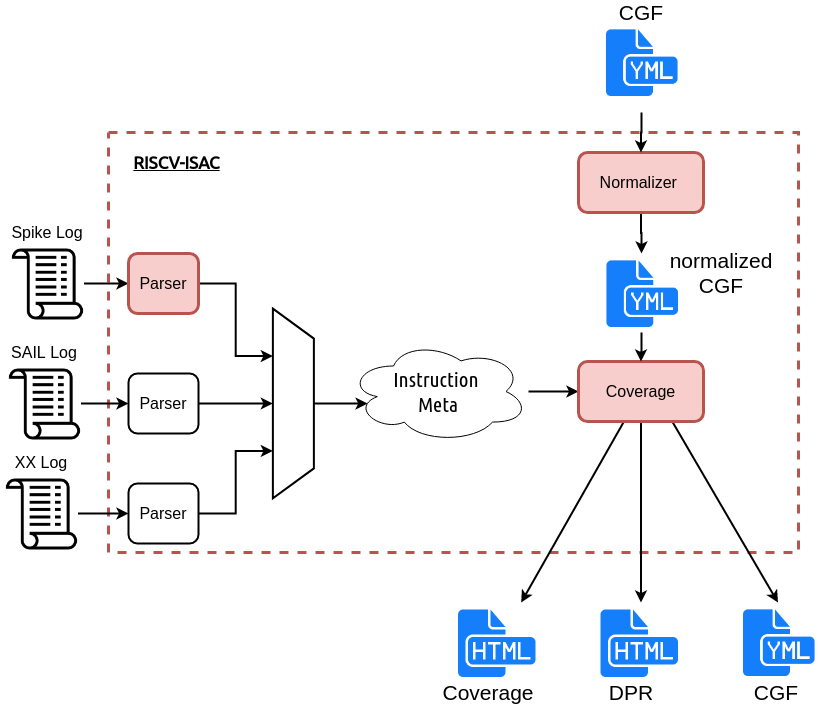
\includegraphics
      [height=.5\textheight]
      {figures/riscv-isac-a.png}
    \end{stampbox}
    \caption{RISCV-ISAC 主组件}
  \end{figure}
  \note<1>[item]{Cover Group Format:感兴趣的覆盖点以直观的 YAML 格式捕获。CGF 文件通常由单个数据集节点和多个覆盖组组成。每个覆盖组可以为不同的指令集定义多个覆盖点。 目前仅支持操作数寄存器和操作数值的叉积。
  \item Execution Trace Format:RISCV-ISAC 需要在 RISC-V 目标(ISS 或 RTL)上运行的测试/应用程序的执行跟踪作为输入。 RISCV-ISAC 使用此跟踪来分析所覆盖的覆盖点。 RISCV-ISAC 中要使用或支持的执行跟踪需要满足以下条件:模型提交/执行的每条指令(可以是 ISS 或 RTL)都应按照提交的顺序捕获为日志中的条目。每个指令条目必须包含指向该指令开头的程序计数器;  每个指令条目必须包含已提交/执行的指令的十六进制编码。每个指令条目还必须包括由于该指令的执行而发生的任何架构状态更新。例如,更新的目标寄存器、修改的 csr、写入的内存区域等。每个指令条目可以跨越多行,每条指令的信息必须可以通过正则表达式检索。指令的助记符是可能的,也应该提供。
  }
  \note<2>[item]{Parser-Module: 解析器模块旨在解析执行跟踪以提取基于每条指令提交的信息。 给定遵循上述格式的执行跟踪,解析器模块能够推导信息并将其提取到公共指令类对象中。 然后将该对象传递到覆盖模块以进行覆盖点分析。随着解析器模块与覆盖模块解耦,对解析不同执行跟踪格式的支持可以轻松集成到 RISCV-ISAC 中。目前支持以下 RISC-V 模型的执行跟踪SAIL;SPIKE.
  \item Normalizer-Module: 输入 CGF 文件中定义的覆盖点可能包含抽象函数.规范化模块负责将这些抽象函数展开到各个覆盖点,并生成覆盖模块使用的规范化 CGF 文件。
  }
  \note<3>[item]{Coverage Module: 覆盖率模块负责执行覆盖率分析并生成 YAML 和 HTML 报告。 覆盖模块维护 RISC-V 的简单架构状态,如 PC、整数寄存器文件等。该状态根据执行跟踪中遇到的指令进行更新。每次解析器呈现指令类对象时,覆盖模块都会检查规范化的 CGF 文件是否有任何覆盖点被该特定指令命中。 一条指令可以命中多个覆盖点。覆盖模块还允许将覆盖范围限制到测试的特定区域。 这些区域由用户根据测试中可用的标签指定。 覆盖模块使用这些标签和 elf 来推断确切的地址范围。覆盖模块可以通过 --cov-label (-l) 参数进一步限制为仅收集 CGF 文件中指定的某些覆盖组的覆盖范围。覆盖模块还可以提供数据传播报告,该报告捕获覆盖点是如何将有助于它们的指令存储在存储区域中的。 这在创建基于签名的测试时特别有用。 然而,此功能需要指定内存区域的标签,类似于使用 --sig-label 参数指定测试区域的方式。覆盖模块在执行结束时生成 4 个工件。第一个是更新的 CGF 文件,其中添加了每个覆盖点的频率。 当合并不同运行中的多个覆盖点时,此文件非常有用。基于 YAML 的报告,捕获详细的高级覆盖点比率。基于 HTML 的报告捕获与 YAML 相同的信息;Markdown 格式的数据传播报告。 仅当签名/数据区域被指定为参数时才可用。}
\end{frame}

\begin{frame}
  \frametitle{RISC-V ISAC 合并组件}
  \begin{figure}
    \centering
    \begin{stampbox}
      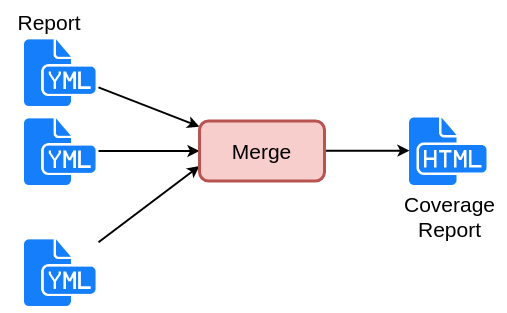
\includegraphics
      [height=.5\textheight]
      {figures/riscv-isac-b.png}
    \end{stampbox}
    \caption{RISCV-ISAC 合并组件}
  \end{figure}
  \note{RISCV-ISAC 还提供了一个简单的合并模块,可以合并多个 CGF 报告以创建单个报告。 这对于为整套测试创建覆盖率报告非常有用。}
\end{frame}

\makebottom

\end{document}